\chapter{Numeri casuali}

\subsection{Introduzione}

In molte applicazioni di analisi numerica è necessario disporre di sequenze di numeri casuali. In realtà i computer non producono numeri casuali, generano sequenze \emph{pseudo-casuali}, cioè successioni determinate da algoritmi deterministici che imitano alcune proprietà statistiche della casualità.

In linea di principio esistono algoritmi che sfruttano sorgenti fisiche per produrre numeri "realmente" (?) casuali, ma nella maggior parte delle applicazioni numeriche si utilizzano generatori pseudo–casuali.

Un generatore di numeri casuali deve produrre sequenze che siano, almeno dal punto di vista statistico, il più possibile indipendenti. Poiché l'algoritmo che produce tali numeri è deterministico, l'obiettivo è costruire procedure che simulino bene il comportamento di una successione indipendente.

Un punto importante è che il grado di ``casualità'' richiesto dipende fortemente dall'applicazione. In alcune simulazioni fisiche o nei metodi Monte Carlo sono richieste proprietà statistiche molto rigorose.

Un riferimento classico sull'argomento è

\begin{quote}
	D. E. Knuth, \emph{Seminumerical Algorithms}, volume 2 di \emph{The Art of Computer Programming}, Addison-Wesley (1981).
\end{quote}

\paragraph*{Considerazioni sui generatori}
Quando si utilizza un generatore di numeri pseudo–casuali è sempre opportuno mantenere un atteggiamento critico nei confronti dei risultati prodotti. In altre parole, bisogna sempre controllare che il generatore non introduca correlazioni indesiderate o artefatti statistici.

Un criterio empirico utile è il seguente: se due generatori diversi producono risultati significativamente differenti per lo stesso esperimento numerico, è probabile che almeno uno dei due presenti problemi.

\begin{quote}
	\emph{``Be suspicious. Once you've been suspicious, stop and be suspicious again.''}\\
	\hfill - Riccardo Mannella
\end{quote}

\vspace{0.5cm}
\subsection{Generatori congruenziali lineari}

Uno dei generatori più elementari e diffusi è il \emph{linear congruential generator}. La sequenza viene costruita tramite la relazione ricorsiva:

\[
x_{n+1} = a x_n + c \pmod m .
\]

Qui $a$ è il moltiplicatore, $c$ è l'incremento, $m$ è il modulo. Scelti $a,\, c,\, m$ ed un '\emph{seed}' $x_n$, la sequenza è continua da sé in modo del tutto deterministico.

Questo tipo di generatore ha il vantaggio di essere molto veloce e di poter essere implementato con grande efficienza anche a basso livello.

Tuttavia presenta alcuni limiti importanti. Le sequenze generate possono mostrare correlazioni interne. Innanzitutto perché la successione può assumere solamente valori fra 0 ed $m-1$

In particolare, se si rappresentano graficamente i punti $(x_n, x_{n+1}, \dots, x_{n+k-1})$ in uno spazio $k$-dimensionale, si osserva che tali punti non riempiono uniformemente lo spazio, ma si dispongono su un insieme di iperpiani.

\begin{multicols}{2}

Più precisamente, i punti generati occupano uno spazio di dimensione $k-1$ e il numero massimo di tali piani è al più $m^{1/k}$, per questo si scelgono sempre alti valori di $m$ per non vedere la periodicità.

Per esempio, scegliendo $m = 2^{32}\,, \text{ e } k = 3\, ,$ si ottiene $m^{1/k}\, \approx\, 1600$ .

Altri esempi con $k=3$:
\begin{itemize}
	\item per $a=421\, ,\, c=1663\, ,\, \text{e } m=7875$, 100 punti e $m^{1/k}\, \approx\, 19.9$;
	\item per $a=4096\, ,\, c=150889\, ,\, \text{e } m=714025$, 10'000 punti e $m^{1/k}\, \approx\, 63.8$.
\end{itemize}

Questo significa che i punti tridimensionali generati dal metodo si dispongono su un numero relativamente limitato di piani, evidenziando quindi una struttura geometrica non desiderata nella sequenza pseudo–casuale.

\begin{figure}[H]
	\centering
	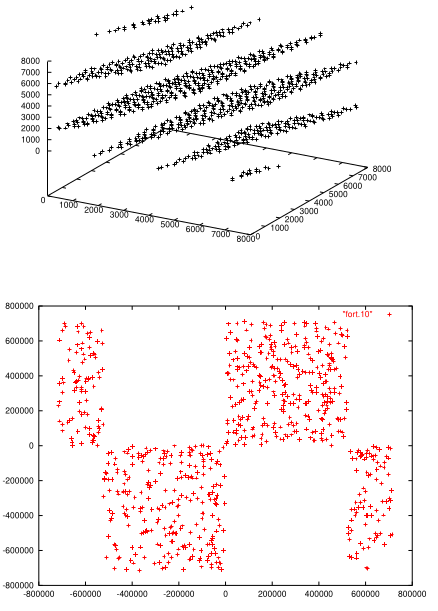
\includegraphics[width=6.5cm]{img/random1.png}
	\label{random 1}
	\caption{ Come si dispongono i punti della successione pseudo-casuale? si nota l'emergere di iperpiani affini che indicano correlazione statistica. La rappresentazione è tridimensionale perché $k=3$. Gli assi rappresentano i punti $(x_n, x_{n+1}, x_{n+3-1})$. }
\end{figure}

\end{multicols}

La rappresentazione grafica mostra chiaramente che i punti non riempiono uniformemente lo spazio tridimensionale, ma si dispongono su un insieme relativamente piccolo di piani.


\vspace{0.5cm}
\subsection{Combinazione di generatori}

Una possibile strategia per migliorare le proprietà statistiche dei generatori congruenziali consiste nel combinare più generatori tra loro.

Un esempio è la routine \texttt{RAN1.F}, che combina tre metodi congruenziali differenti. In particolare, vengono utilizzati generatori distinti per i bit più significativi, per quelli meno significativi e per una procedura di \emph{reshuffling} della sequenza.

Se la velocità di esecuzione è il fattore principale, è possibile utilizzare una combinazione più semplice di due generatori congruenziali. Questa strategia è adottata nella routine \texttt{RAN2}. Tuttavia, in questo caso il generatore tende a campionare una porzione più limitata dello spazio delle configurazioni.

\lstinputlisting[style=Fortranstyle,
	caption={RAN1.f90, combinazione di generatori congruenziali, esempio ispirato al \emph{"Numerical Recipes"} di Press, Teukolsky, Vetterling, Flannery. Nota bene: questa è solamente una routine, per essere utilizzata va chiamata},
	label={lst:combinazione generatori}]{RAN1.f90}


\vspace{0.5cm}
\subsection{Generatori basati su sistemi caotici}

Un approccio alternativo consiste nello sfruttare il comportamento caotico di alcuni sistemi dinamici.

L'idea è quella di utilizzare un sistema dinamico deterministico che presenti una dinamica caotica controllata, e impiegare la successione dei suoi stati come sequenza pseudo–casuale.

\begin{multicols}{2}

Un esempio classico è dato dalla mappa logistica:

\begin{equation}
	\label{logistic map eq}
	x_{n+1} = \lambda x_n (1 - x_n)\ \ .
\end{equation}

Al variare del parametro $\lambda$ il sistema in eq.(\ref{logistic map eq}) mostra un comportamento sempre più complesso, fino a entrare in regime caotico (come si vede in figura).


\begin{figure}[H]
	\centering
	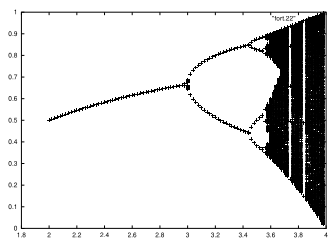
\includegraphics[width=6.5cm]{img/logisticcurve.png}
	\label{logistic map img}
	\caption{ La \href{https://youtu.be/ovJcsL7vyrk?si=zD5sAjndwQtBor5K}{curva logistica}, sembra di essere tornati a \href{https://youtu.be/j07YwnzGnII?si=a3Tg0EYx67gUO86X}{lezione da Paolini}, wow }
\end{figure}

\end{multicols}

Tuttavia l'utilizzo diretto di sistemi caotici come generatori pseudo–casuali presenta diversi problemi pratici. In particolare, è necessario stabilire quanto il comportamento caotico del sistema sia effettivamente adeguato per simulare una sequenza statisticamente indipendente.


\vspace{0.5cm}
\subsection{Generatori come sistemi dinamici a molti stati}

Un modo più efficace per costruire generatori pseudo–casuali consiste nel progettare sistemi dinamici con un numero elevato di stati interni.

L'idea è quella di costruire una macchina a molti stati in cui il valore successivo della sequenza dipende da una combinazione di stati precedenti. Questo schema può essere rappresentato come una rete di variabili interne che interagiscono tra loro attraverso operazioni di somma o sottrazione.

Questa idea è alla base dei cosiddetti algoritmi \emph{add and carry} oppure \emph{subtract and carry}. Tra i generatori di questo tipo si trovano, ad esempio,

\begin{itemize}
	\item la routine \texttt{RAN3}: si mantiene una tabella di numeri precedenti e si genera il nuovo valore come differenza di due elementi della sequenza (In forma semplificata: $x_n=x_{n−j}-x_{n−k}$);
	
	\item il generatore \texttt{rcarry}: questo è un generatore della famiglia subtract-with-carry. È simile a quello precedente ma introduce una variabile aggiuntiva chiamata carry (l'idea è: $x_n=x_{n−r}-x_{n−s}-c$).
\end{itemize}

Questi algoritmi presentano in genere periodi di ripetizione molto lunghi e buone proprietà statistiche (risolvendo parzialmente il problema della struttura geometrica in iperpiani).




\section{Generazione di distribuzioni non uniformi}

\subsection{Dal caso uniforme a una distribuzione arbitraria}

Dopo aver costruito un generatore di numeri pseudo--casuali uniformi, il problema successivo consiste nel produrre variabili aleatorie con una distribuzione assegnata. In altre parole, dato un generatore che fornisce variabili uniformi, vogliamo ottenere campioni distribuiti secondo una densità prefissata.

Sia dunque $x$ una variabile casuale distribuita uniformemente in un certo intervallo, con densità $p(x)$, e supponiamo di voler costruire una nuova variabile $y$ con densità $p(y)$. La relazione fondamentale tra le due densità si ottiene imponendo l'\underline{invarianza della probabilità} sotto trasformazione di variabile.
Si ha infatti $|p(y)\,dy| = p(x)\,dx$, da questa relazione segue immediatamente che:

\[
p(y) = p(x)\left|\frac{dx}{dy}\right| .
\]

Questa formula esprime il fatto che la densità della nuova variabile dipende dalla densità di partenza e dal modo in cui la trasformazione $x \mapsto y$ dilata o contrae gli intervalli.

Il problema centrale diventa allora quello di determinare una trasformazione opportuna tra $x$ e $y$. Ciò si riconduce a risolvere
$\frac{dx}{dy} = f(y)$ .

In sostanza, assegnata la distribuzione voluta, si cerca una funzione di trasformazione tale che la variabile uniforme iniziale venga mappata nella nuova variabile con la densità desiderata.

%
%
%
\vspace{0.5cm}
\subsection{Metodo della funzione cumulativa inversa}

Il procedimento precedente si chiarisce riscrivendo la trasformazione in termini di funzione integrale della densità.

Ricordando la relazione $\frac{dx}{dy} = f(y)$ ed integrando rispetto a $y$, si ottiene

\[ x = F(y)\ \ ,\]

dove la funzione $F(y)$ è data, a meno di costanti additive o di opportune normalizzazioni, dall'integrale della densità:

\[ F(y) = \int p(y)\,dy\ \ . \]

Se la funzione $F$ è invertibile, allora si può esprimere $y$ in funzione di $x$ come

\[
y(x) = F^{-1}(x).
\]

Questo è il contenuto essenziale del metodo della trasformazione inversa: si genera una variabile uniforme $x$, si costruisce la funzione cumulativa associata alla densità desiderata, e infine si ottiene la variabile distribuita secondo $p(y)$ applicando l'inversa della cumulativa.

Il metodo funziona quindi molto bene quando l'inversa dell'integrale di $p(y)$ è disponibile in forma esplicita, oppure può essere calcolata numericamente in modo efficiente. 




\subsubsection{Esempio: distribuzione esponenziale}

Un esempio particolarmente importante è quello della distribuzione esponenziale. Si consideri la trasformazione

\[
y(x) = -\ln x .
\]

Se $x$ è uniforme nell'intervallo $(0,1)$, allora

\[
\frac{dx}{dy} = -e^{-y},
\qquad
\left|\frac{dx}{dy}\right| = e^{-y}.
\]

Poiché la densità di $x$ è uniforme, cioè costante su $(0,1)$, dalla relazione generale

\[
p(y)\,dy = p(x)\left|\frac{dx}{dy}\right|dy
\]

segue che, a meno della costante uniforme $p(x)$, la densità di $y$ è

\[
p(y)\,dy = e^{-y}\,dy .
\]

Si ottiene dunque la distribuzione esponenziale. 


%
%
%
\subsubsection{Interpretazione geometrica del metodo}

Ripartiamo da $F(y) = \int p(y)\,dy$ ; si osserva che la variabile uniforme $x$ viene ottenuta come valore della cumulativa associata a $y$. Invertendo questa relazione, si ha ancora

\[
y(x) = F^{-1}(x).
\]

Geometricamente, la funzione $F(y)$ cresce dal valore minimo al valore massimo della probabilità cumulata. Se si estrae un numero uniforme $x$ tra $0$ e $1$, lo si può interpretare come un livello di probabilità cumulata; il valore corrispondente di $y$ si ottiene leggendo sull'asse orizzontale il punto in cui la cumulativa raggiunge proprio quel livello.

In altre parole, il metodo della trasformazione inversa trasforma una distribuzione uniforme della probabilità cumulata in una distribuzione non uniforme della variabile fisica.

\subsubsection{Esempio: tempi di decadimento}

Sappiamo che quando i nuclei decadono hanno una densità di probabilità $p(t)\,=\, \lambda e^{-\lambda \, t}$ di decadere, nel senso che $p(t)\,dt$ è la probabilità di decadere nell'intervallo di tempo $t$, $t+dt$; inoltre sappiamo che la cumulativa di questa probabilità, 
\[F(t^*)\,=\, P(T<t^*)\,=\, \int_0^{t^*} p(T)\, dT\,=\, 1-e^{-\lambda \, t^*}\]
ci dà invece la probabilità che il nucleo sia decaduto prima dell'istante $t^*$.

Partiamo quindi dalla probabilità accumulata ed scegliamo un valore $u\in[0,\, 1]$, per poi porre l'uguaglianza $1-e^{-\lambda \, t^*}=u$ che invertita restituisce $t^*=-\frac{1}{\lambda}\, \log(1-u)$. Questo passaggio equivale ad estrarre una percentuale di nuclei decaduti e a chiedersi 'quanto tempo $t^*$ si dovrebbe aspettare per vedere una frazione $u$ di nuclei decadere?'.

Nonostante il processo sia poissoniano ed ogni atomo decada dopo un tempo diverso, si può continuare ad estrarre valori $u$ quanti sono gli atomi e questo ci permette trovando tutti i tempi corrispondenti di ricostruire la distribuzione esponenziale iniziale.

%
%
%
\vspace{0.5cm}
\subsection{Trasformazioni in più dimensioni}

Il metodo di trasformazione non è limitato al caso unidimensionale, ma si estende anche a distribuzioni in più variabili.

Se $(x_1,x_2,\dots)$ è un vettore di variabili di partenza e $(y_1,y_2,\dots)$ è il nuovo vettore di variabili, allora la relazione tra le densità è regolata dal determinante jacobiano della trasformazione:

\[
p(y_1,y_2,\dots)\,dy_1dy_2\cdots
=
\left|
\frac{\partial(x_1,x_2,\dots)}{\partial(y_1,y_2,\dots)}
\right|
p(x_1,x_2,\dots)\,dy_1dy_2\cdots .
\]

Questa espressione generalizza direttamente la formula unidimensionale.

Anche qui il significato è lo stesso: la densità si modifica in funzione della deformazione locale dei volumi elementari operata dalla trasformazione.


\vspace{0.5cm}
\subsection{Generazione di distribuzioni gaussiane: metodo di Box-Muller}

Un'applicazione molto importante del caso multidimensionale è la generazione di variabili gaussiane: il metodo di \href{https://www.taygeta.com/random/gaussian.html}{Box-Muller}, che permette di ottenere due variabili gaussiane indipendenti a partire da due variabili uniformi indipendenti.

Si considerino due variabili uniformi indipendenti $x_1$ e $x_2$, entrambe distribuite uniformemente in $(0,1)$. Si definiscono allora le nuove variabili

\[
y_1 \,=\, \sqrt{-2\ln x_1}\,\cos(2\pi x_2) \,=\, r\cos\theta,
\]

\[
y_2 \,=\, \sqrt{-2\ln x_1}\,\sin(2\pi x_2) \,=\, r\sin\theta.
\]

Queste formule costituiscono la trasformazione di Box--Muller. Le due variabili uniformi $x_1$ e $x_2$ vengono reinterpretate come variabili ausiliarie che costruiscono, rispettivamente, il raggio e l'angolo in coordinate polari nel piano delle variabili gaussiane. In particolare, $r = \sqrt{-2\ln x_1}$ e $\theta = 2\pi x_2$ .

Questa trasformazione è progettata in modo tale che la densità congiunta di $(y_1,y_2)$ risulti gaussiana e radialmente simmetrica, così da avere una routine che trasformi due variabili indipendenti distribuite uniformemente in due variabili distribuite gaussianamente.

\begin{figure}[H]
	\centering
	\label{box-muller}
	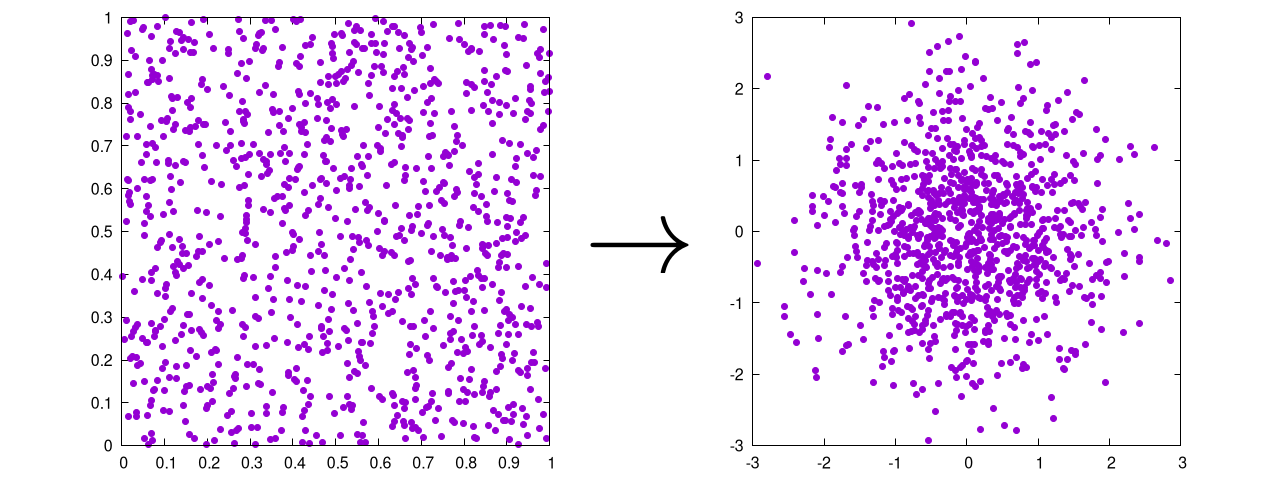
\includegraphics[width=10cm]{img/cartesian_rand_transform.png}
	\caption{Immagine presa da \href{https://www.algorithm-archive.org/contents/box_muller/box_muller.html}{QUI  <--}}
\end{figure}


\paragraph{Calcolo del Jacobiano nella trasformazione di Box-Muller}

Per giustificare il metodo bisogna analizzare lo jacobiano della trasformazione. Partiamo dalla trasformazione sopra presentata, con definizioni di $y_1,\, y_2,\, r,\, \theta$. Si ricava:

\[
x_1 = e^{-r^2/2},
\qquad
x_2 = \frac{\theta}{2\pi}.
\]

Poiché $x_1$ e $x_2$ sono uniformi e indipendenti, la loro densità congiunta è costante nel quadrato unitario: $p(x_1,x_2)=1,
\quad 0<x_1<1,\ 0<x_2<1$.


Ora, il passaggio da $(x_1,x_2)$ a $(r,\theta)$ produce il fattore jacobiano

\[\left|
\begin{matrix}
	\displaystyle\frac{\partial x_1}{\partial r} & \displaystyle\frac{\partial x_1}{\partial \theta}\\[4pt]
	\displaystyle\frac{\partial x_2}{\partial r} & \displaystyle\frac{\partial x_2}{\partial \theta}
\end{matrix}
\right|\ =\ 
\left|
\begin{matrix}
	-r e^{-r^2/2} & 0\\[4pt]
	0 & \frac{1}{2\pi}
\end{matrix}
\right|.\]

si ottiene $\displaystyle\left|\frac{\partial(x_1,x_2)}{\partial(r,\theta)}\right|\,=\,\displaystyle\frac{r}{2\pi}\, e^{-r^2/2}$ .


Per passare poi da coordinate polari a coordinate cartesiane si usa il noto elemento di area $dy_1\,dy_2 = r\,dr\,d\theta$, cioè $dr\,d\theta = \displaystyle\frac{1}{r}\,dy_1\,dy_2$.

Combinando i due passaggi, si trova che la densità di $(y_1,y_2)$ è proporzionale a $\displaystyle\frac{r}{2\pi}e^{-r^2/2}\cdot \frac{1}{r}\, =\,\displaystyle\frac{1}{2\pi}e^{-r^2/2}$.
Poiché $r^2 = y_1^2 + y_2^2$, segue che:

\[
P(y_1,y_2)=\frac{1}{2\pi}\exp\left(-\frac{y_1^2}{2}-\frac{y_2^2}{2}\right).
\]

Questa è precisamente la distribuzione normale bidimensionale standard 
con componenti indipendenti.

%
%
%
%\vspace{0.5cm}
\subsubsection{Osservazione conclusiva su questa parte}

Riassumendo, il principio generale è il seguente: una volta ottenute variabili uniformi affidabili, si possono costruire distribuzioni non uniformi applicando trasformazioni opportune. Nel caso unidimensionale il punto chiave è l'inversione della cumulativa; nel caso multidimensionale entra in gioco il determinante jacobiano della trasformazione.

Questo quadro teorico prepara direttamente al metodo di \emph{rejection}, che diventa essenziale quando l'inversa della cumulativa non è disponibile in forma trattabile.

%
%
%
\vspace{0.5cm}
\section{Rejection method}

Il metodo del rifiuto permette di generare distribuzioni non uniformi senza richiedere il calcolo esplicito dell'integrale della densità.

Si consideri una distribuzione di probabilità desiderata $p(x)$, e una funzione $f(x)$ tale che $f(x) > p(x) \quad \forall\ x$ , l'idea è utilizzare una coppia di variabili casuali uniformi per campionare la distribuzione $p(x)$.

Si procede nel seguente modo:

\begin{itemize}
	\item si estrae un valore $x_s$ uniformemente distribuito nel dominio;
	\item si estrae una seconda variabile casuale $x_1$ uniforme tra $0$ e $f(x_s)$;
	\item si accetta $x_s$ se vale la condizione $x_1 < p(x_s)$
\end{itemize}

Se la condizione non è soddisfatta, il punto viene rifiutato e si ripete la procedura. Questo metodo non richiede la conoscenza della funzione cumulativa, ma soltanto una funzione $f(x)$ che sovrastimi $p(x)$.

\paragraph{Interpretazione geometrica:}

Il metodo può essere interpretato geometricamente. Si consideri il grafico delle funzioni $p(x)$ e $f(x)$, con $f(x)$ tale che $f(x) \ge p(x)$

\begin{multicols}{2}
\begin{figure}[H]
	\label{rejection img}
	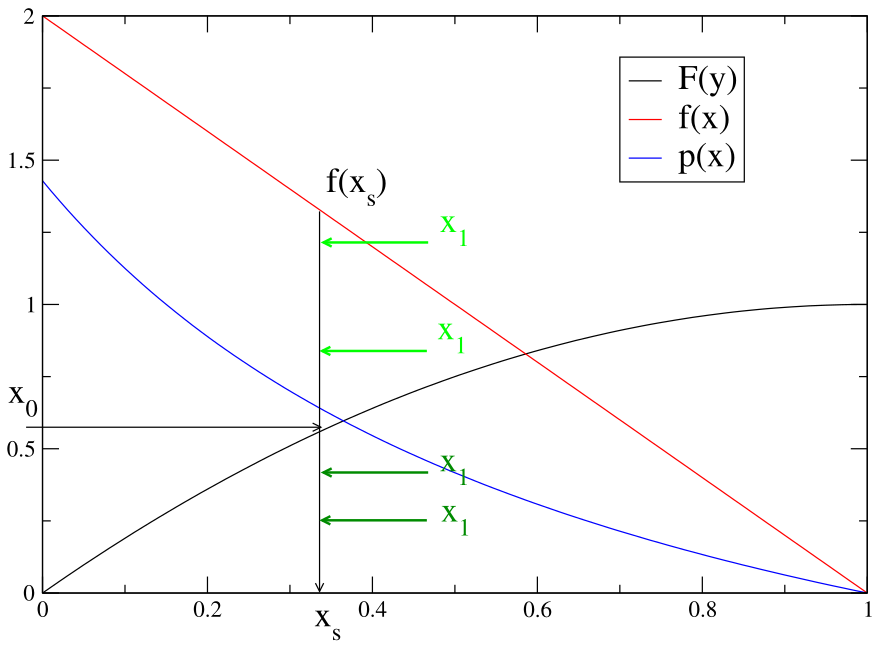
\includegraphics[width=6.9cm]{img/rejection.png}
	\caption{rappresentazione grafica del \emph{rejection method}}
\end{figure}

Si generano punti uniformemente nella regione delimitata da $f(x)$.

Un punto viene accettato se cade sotto la curva $p(x)$.

In questo modo, i punti accettati risultano distribuiti secondo la densità desiderata.

In fig.(\ref{rejection img}), i punti accettati sono quelli che cadono sotto $p(x)$, mentre gli altri vengono scartati.
\end{multicols}

%
%
%
\subsection{Metodo del rifiuto per la distribuzione Gamma}

La distribuzione Gamma di ordine intero $a > 0$ rappresenta la distribuzione del tempo di attesa per il verificarsi del $a$-esimo evento in un processo di Poisson con valore medio unitario ed è data da:

\begin{equation}
	p_a(x)\,dx \ =\
	\frac{x^{a-1} e^{-x}}{\Gamma(a)}\,dx\ \ ,
	\qquad x>0\ \ ,
\end{equation}


Per valori piccoli di $a$, è possibile generare direttamente la distribuzione come somma di variabili esponenziali indipendenti.

Questo equivale a calcolare il prodotto di $a$ variabili casuali uniformi e successivamente prendere il logaritmo.

Per valori più grandi di $a$, la distribuzione assume una forma a campana: con massimo circa in $x \approx a$ e larghezza dell'ordine $\sqrt{a}$

%
\subsubsection{Funzione di confronto}

Per applicare il metodo del rifiuto, si introduce una funzione di confronto.

Una scelta conveniente che si rivela utile è la distribuzione di Lorentz:

\begin{equation}
	\label{Lorentziana}
	p(y)\,dy =
	\frac{1}{\pi (1 + y^2)}\,dy
\end{equation}

Integrandola si ottiene

\begin{equation}
	F(y) = \int p(y)\,dy = \frac{1}{\pi} \arctan(y)
\end{equation}

\begin{multicols}{2}
	
%
\subsubsection{Funzione di maggiorazione}

Si introduce una funzione $f(x)$ della forma

\begin{equation}
	f(x)\ =\
	\frac{c_0}{1\, +\, (x - x_0)^2 / a_0^2}
\end{equation}

Questa funzione deve essere scelta in modo tale che $f(x) \ge p(x)$ e che il prodotto $a_0\, c_0$ sia il più piccolo possibile, al fine di minimizzare il numero di rifiuti.

\begin{figure}[H]
	\centering	
	\label{gamma+lorentz}
	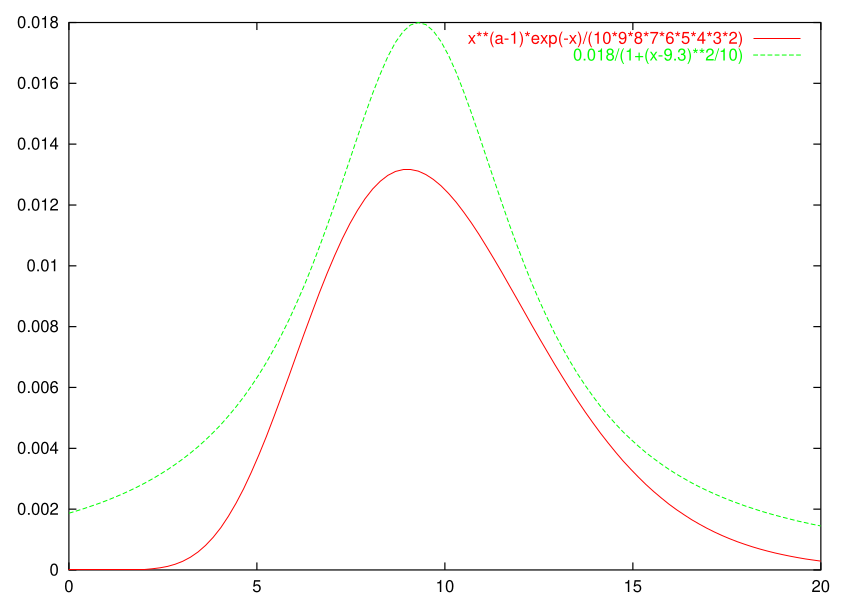
\includegraphics[width=6cm]{img/gamma_function.png}
	\caption{\emph{Gamma function} in rosso, mentre in verde si vede la lorentziana, funzione di maggiorazione $f(x)$.}
\end{figure}
\end{multicols}

\subsubsection{Algoritmo}

Si genera una variabile uniforme $u \in [0,1]$ e si pone $x = a_0 \tan(\pi u) + x_0$ cioè $x = f^{-1}(y)$.

Successivamente si verifica la condizione di accettazione (rejection test).

Questo procedimento è implementato, ad esempio, nella routine \texttt{GAMDEV}.

\lstinputlisting[style=Cstyle,
	caption={Implementazione del metodo GAMDEV},
	label={lst:gamma rejection}]{GAMDEV.c}


%
%
%
\vspace{0.5cm}
\section{Integrazione Monte Carlo}

Il metodo di integrazione Monte Carlo è strettamente collegato al metodo del rifiuto.

Esso permette di stimare integrali multidimensionali mediante campionamento casuale.

In uno spazio $n$-dimensionale, dato un insieme di $N$ punti $x_i$, vale la stima

\begin{equation}
	\int_V f\,dV\ \approx\ V \langle f \rangle\, \pm\, V\, \sqrt{\frac{\langle f^2 \rangle - \langle f \rangle^2}{N}}
\end{equation}

dove

\begin{equation}
	\langle f^n \rangle =
	\frac{1}{N} \sum_{i=1}^N f^n(x_i)
\end{equation}

\begin{multicols}{2}
\subsubsection{Interpretazione}

L'idea è quella di incorporare una regione difficile da campionare all'interno di una regione più semplice, dalla quale è possibile estrarre punti uniformemente.

Successivamente si utilizza il campionamento casuale per stimare l'integrale.

Il metodo può essere scritto in molti modi diversi in base a in quante dimensioni stiamo campionando, in quale spazio estraiamo i nostri punti e che forma ha la funzione, ma il concetto rimane sempre questo.

\begin{figure}[H]
	\centering
	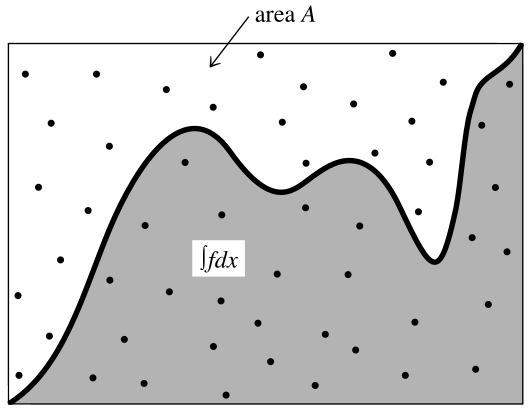
\includegraphics[width=7cm]{img/MonteCarloIntegration.png}
	\label{monte carlo}
	\caption{Esempio visuale preso da "\emph{Numerical Recipes in C}". L'integrale della funzione $f$ è stimato come l'area del rettangolo A moltiplicata per la frazione di punti che si trova sotto la curva $f$}
\end{figure}

\end{multicols}


\subsubsection{Esempio: area di un cerchio}

Si consideri il calcolo dell'area di un cerchio unitario.

Si definisce una funzione

\begin{equation}
	f =
	\begin{cases}
		1 & \text{all'interno del cerchio} \\
		0 & \text{all'esterno}
	\end{cases}
\end{equation}

Il volume della regione di campionamento è V = 4, la stima dell'area è $\int_V f\,dV \approx V \langle f \rangle$


\begin{multicols}{2}
Per $N = 1000$ si ottiene

\[\begin{aligned}
	\langle f \rangle &=\ 0.797\\
	\text{area} &=\ 3.19 \pm 0.05
\end{aligned}\]

Per $N = 10^6$:

\[\begin{aligned}
	\langle f \rangle &=\ 0.78616\\
	\text{area} &=\ 3.145 \pm 0.005
\end{aligned}\]

\begin{figure}[H]
	\centering
	\label{aa}
	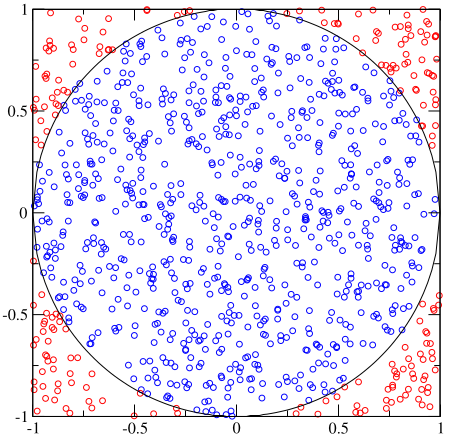
\includegraphics[width=5cm]{img/pie.png}
	\caption{Integrale Monte Carlo dell'area di un cerchio}
\end{figure}
\end{multicols}

%
\subsubsection{Esempio: disco con foro}

Si consideri un disco di raggio 1 con un foro di raggio 0.5 centrato nel punto $(0.5,0)$.

Si vogliono calcolare:

\begin{equation}
	x_{cm} = \frac{\int x\,dV}{\int dV}
\end{equation}

\begin{equation}
	I_{0,0} = \int (x^2 + y^2)\,dV
\end{equation}


\begin{multicols}{2}

Le funzioni da integrare sono:

\begin{itemize}
	\item $f_x = x$ all'interno della regione, zero fuori;
	\item $f_y^2 = y^2$, ecc.
\end{itemize}

Per $N = 10^6$ si ottiene:

\[\begin{aligned}
	x_{cm} &=\ -0.393\ \pm\ 0.004\\
	y_{cm} &=\ -0.000\ \pm\ 0.005\\
	I_{0,0} &\approx\ 1.275
\end{aligned}\]

\begin{figure}[H]
	\centering
	\label{aaa}
	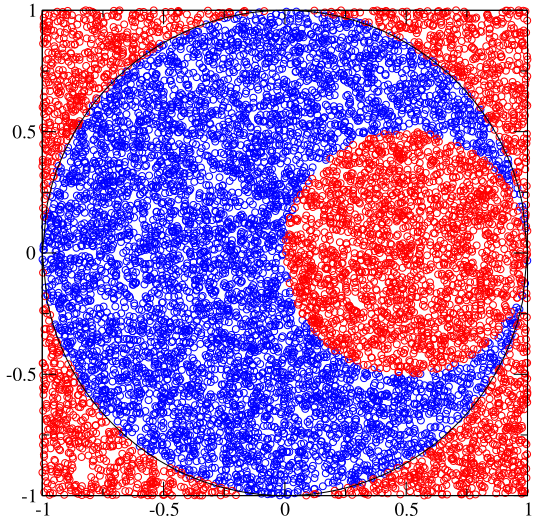
\includegraphics[width=6cm]{img/MCintegral.png}
	\caption{Integrale Monte Carlo dell'area di un cerchio forato}
\end{figure}
\end{multicols}

\lstinputlisting[style=Pythonstyle,
	caption={Esercizio di integrazione Monte Carlo del disco bucato in Python, scritta da ChatGpt 5.3},
	label={lst:gamma rejection}]{MonteCarloIntegration-HoledDisk.py}
